\documentclass{amsart}

\usepackage{amsmath}
\usepackage{amsfonts}
\usepackage{amssymb}
\usepackage{graphicx}

\title{Problem Set 1}
\author{Mark Ditsworth}

\begin{document}
	\maketitle
	\section{Linear Algebra}
	\subsection{Problem 1}
	Show that if $M\in \mathbb{R}^{n\times n}$ is a symmetric matrix and $d \leq n$, then $U \in \mathbb{R}^{n\times d}$ and $U^T U=I_{d\times d}$,
	\[
	\max_d \text{Tr} \left(U^T M U\right) = \sum_{k=1}^{d}\lambda_{k}^{(+)}
	\]
	where $\lambda_{k}^{(+)}$ is the $k$th largest eigenvalue of $M$.\\
	\\
	Since $M$ is symmetric, we have the singular value decomposition (SVD)
	\[
	M = U D^2 U^T
	\]
	where $D$ is a diagonal matrix with values corresponding to the eigenvalues of $M$, in order of magnitude. Since $U^TU = I \Rightarrow U^T = U^{-1}$, we have
	\[
	U^{-1}M(U^T)^{-1} = D^2
	\]
	\[
	U^TMU = D^2
	\]
	Therefore, $\text{Tr} \left(U^T M U\right) =\text{Tr}\left(D^2\right) = \sum_{k=1}^{n}\lambda_k^{(+)}$
	
	In order to maximize this, we can set $d$ such that $\lambda_{d+1}^{(+)}$ is the first occurrence of a negative eigenvalue in the $\lambda_k^{(+)}$ sequence.
	\\
	\section{Estimators}
	\subsection{Problem 2}
	Given $x_1, \dots x_n$ i.i.d samples from a distribution $X$ with mean $\mu$ and covariance $\Sigma$, show that
	\[
	\mu_n = \frac{1}{n}\sum_{k=1}^{n}x_k \qquad,\qquad \Sigma_n = \frac{1}{n-1}(x_k - \mu)(x_k - \mu)^T
	\]
	are unbiased estimators for $\mu$ and $\Sigma$. (Show that $\mathbf{E}[\mu_n]=\mu$ and $\mathbf{E}[\Sigma_n]=\Sigma$)\\
	\\
	\[
	\mathbf{E}[\mu_n] = \mathbf{E}\left[\frac{x_1+\dots+x_n}{n}\right] = 
	\frac{\mathbf{E}[x_1]+\dots+\mathbf{E}[x_n]}{n}=
	\frac{n\mu}{n}=\mu
	\]
	\\
	\[
	\mathbf{E}[\Sigma_n] = \frac{1}{n-1}\sum_{i=1}^{n}
	\mathbf{E}\left[(x_i-\mu_n)(x_i-\mu_n)^T\right]=
	\frac{1}{n-1}\sum_{i=1}^{n}\mathbf{E}\left[((x_i-\mu)-(\mu_n-\mu))((x_i-\mu)-(\mu_n-\mu))^T\right]
	\]
	\[
	=\frac{1}{n-1}\sum_{i=1}^{n}\mathbf{E}\left[
	(x_i-\mu)(x_i-\mu)^T\right]+\mathbf{E}\left[
	(\mu_n-\mu)(\mu_n-\mu)^T\right]-\mathbf{E}\left[
	(x_i-\mu)(\mu_n-\mu)^T\right]-\mathbf{E}\left[
	(\mu_n-\mu)(x_i-\mu)^T\right]
	\]
	\[
	=\frac{1}{n-1}\sum_{i=1}^{n}\mathbf{E}\left[
	(x_i-\mu)(x_i-\mu)^T\right] = 
	\sum_{i=1}^{n}\mathbf{E}\left[
	\frac{(x_i-\mu)(x_i-\mu)^T}{n-1}\right]=
	\mathbf{E}\left[\sum_{i=1}^{n}
	\frac{(x_i-\mu)(x_i-\mu)^T}{n-1}\right]=\Sigma
	\]
	\\
	\section{Random Matrices}
	\subsection{Problem 3}
	Let $W \in \mathbb{R}^{n\times n}$ be a Wigner Matrix, a symmetric random matrix whose diagonal and upper-diagonal entries are independent $W_{ii} \sim \mathbb{N}(0,2)$ and for $i<j$, $W_{ij} \sim N(0,1)$. Show that the distribution of the eigenvalues of $\frac{1}{\sqrt{n}}W$ converge to the semi-circle law of support $[-2,2]$
	\[
	dSC(x) = \frac{1}{2\pi}\sqrt{4-x^2}1_{[-1,1]}(x)
	\]
	\\
	\begin{figure}[h!]
	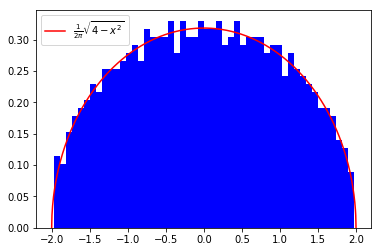
\includegraphics[]{dSC.png}
	\caption{Histogram of eigenvalues for the $\frac{1}{\sqrt{n}}W$ ($n=500$)}
	\end{figure}
	\\
	\subsection{Problem 4}
	Use Slepian's Comparison Lemma to show that for a Wigner matrix $W\in \mathbb{R}^{n \times n}$, where $W_{ij | i\neq j} \sim N(0,1)$ and $W_{ii} \sim N(0,2)$.
	\\
	\[
	\mathbf{E}\left[\lambda_{max}(W)\right] \leq 2\sqrt{n}
	\]
	\\
	\[
	\lambda_{max}(W) = \max_v v^T W v \Rightarrow \mathbf{E}\left[\lambda_{max}(W)\right] = \mathbf{E}\left[\max_v v^t W v\right]
	\]
	\[
	\text{Let } Y_v \ddot{=} \max_v v^T W v 
	\]
	\[
	\text{Define } X_v = v^Tg \qquad g \sim N(0,I_{n\times n})
	\]
	Slepian's Comparison Lemma states that for random variables $X_v$ and $Y_v$, if $\mathbf{E}[X_v]=\mathbf{E}[Y_v]=0$, and $\forall v1, v2 \in V$ s.t. $v1 \neq v2$ $\mathbf{E}[X_{v1}-X_{v2}]^2 \geq \mathbf{E}[Y_{v1}-Y_{v2}]^2$, then
	\[
	\mathbf{E}\left[\max_v Y_v\right] \leq \mathbf{E}\left[\max_v X_v\right]
	\]
	Since $X_v$ and $Y_v$ are both related to Gaussians about 0, the first condition is satisfied. Monte Carlo simulation of $\mathbf{E}[2X_{v1}-2X_{v2}]^2 - \mathbf{E}[Y_{v1}-Y_{v2}]^2$ are shown below; clearly the value is $\geq 0$, thus satisfying the second condition.
	\begin{figure}[h!]
		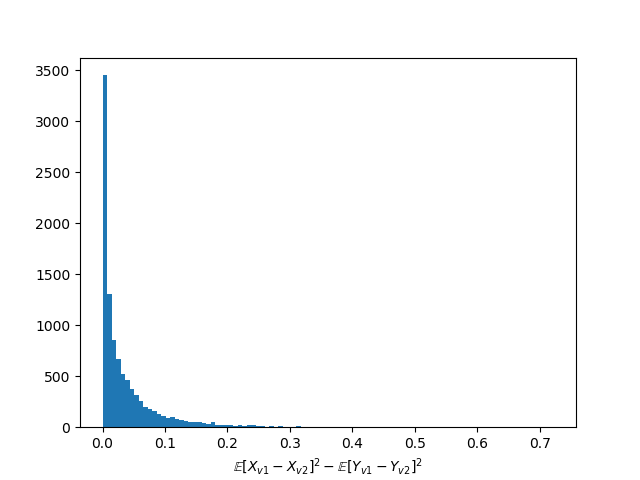
\includegraphics[scale=0.6]{subtract.png}
	\end{figure}
	Therefore, it is sufficient to say that \[\mathbf{E}\left[\max_v Y_v\right] \leq \mathbf{E}\left[\max_v 2X_v\right]\]
	By Jensen's inequality, we have that
	\[
	\mathbf{E}\left[\max_v X_v\right]^2 \leq \mathbf{E}\left[\left(\max_v X_v\right)^2\right]
	\]
	\[
	\mathbf{E}\left[\max_v v^Tg\right]^2 \leq \mathbf{E}\left[\left(\max_v v^Tg\right)^2\right]
	\]
	Since $||v||_2=1$, $v^Tg$ will be maximized when each element of $v$ is equal to $\frac{1}{\sqrt{n}}$. Thus, $max_v v^Tg = \frac{1}{\sqrt{n}}\sum_{i=1}^n g_i$. Since $g$ is standard Gaussian, $\sum_{i=1}^{n}g \leq n$, thus $max_v v^Tg \leq \sqrt{n}$. Therefore, we have 
	\[
	\mathbf{E}\left[\max_v v^Tg\right]^2 \leq n
	\]
	\[
	\mathbf{E}\left[\max_v v^Tg\right] \leq \sqrt{n}
	\]
	and finally
	\[
	\mathbf{E}[\max_v Y_v] = \mathbf{E}[\lambda_{max}(W)] \leq 2\sqrt{n}
	\]
	\subsection{Problem 5}
	Consider the matrix $M = \frac{1}{\sqrt{n}}W + \beta vv^T$ for $||v||_2=1$ and $W$ is a standard Gaussian Wigner Matrix. If $v=e_1$, this is a rank 1 perturbation of a Wigner matrix. Derive the limit of the largest eigenvalue.
	\\
	\section{Diffusion Maps}
	\subsection{Problem 6}
	Derive the 2-D diffusion map embedding for the $n$-node ring graph. If the eigenvalues are complex, try creating real ones using multiplicity of eigenvalues. Is it a reasonable embedding of this graph in two dimensions?
	
	\begin{figure}[h!]
		\centering
		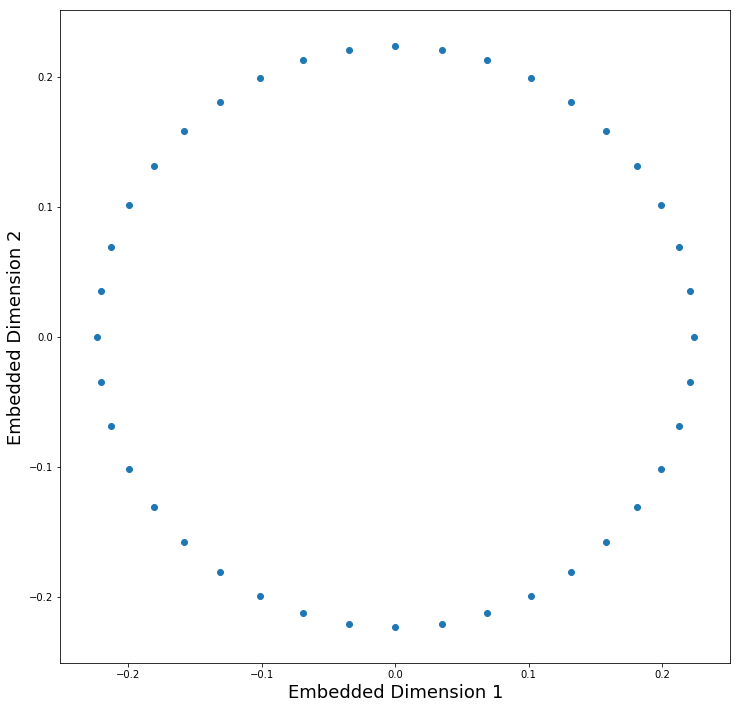
\includegraphics[width=0.8\linewidth]{diffmap.png}
	\end{figure}
\end{document}